\section{Start working with Faces databases}
Once LeNet-5 architecture has been understanding, the used database is changed because the final goal is using a convolutional neural network with different faces databases.\\

\subsection{Using Labeled Faces in the Wild}
With the purpose of reading and working with face images, the Labeled Faces in the Wild (LFW) database is used. Because of that, a script has been developed where images are precessed. All images are pseudo-randomized and grouped in training set (49\% of the total database), testing test (30\% of the total data) and validating set (21\% of the data).\\

To split the data, train\_test\_split function from sklearn.cross\_validation has been used. This function pseudo-randomize the data, so you can repeat the randomized split data in the same way assigning the same seed to the function.\\

For the next experiment, 500 samples are used for each batch, so 13 batches are going to be used for training, 6 for validation and 6 for testing. Images has been resized to 28x28 size, as MNIST digit database available with the code. \\

The parameters has not been changed, but the number of epoch that has been decreased to 12, and the number of neurons at the output of the logistic regression that has been changed from 10 to 5748 (the number of classes or different people).\\

%\begin{itemize}
%\item $learning_rate=0.1, n_epochs=12, nkerns=[20, 50], batch_size=500$
%\item  T.tanh activation function
%\item rng = numpy.random.RandomState(23455)
%\item kernel size = [5,5]
%\item images resized to 28x28
%\item 12 epoch
%\item The number of neurons at the input of the regression class is 10000, and the number of neurons at the output is 5748 (Number of people).
%\end{itemize}
The results obtained are not good, because of the fact that the network has not been optimized to this purpose, the number of epoch should be more and for each class there are a few samples and should be much more.\\

\begin{figure}[htb]
\centering
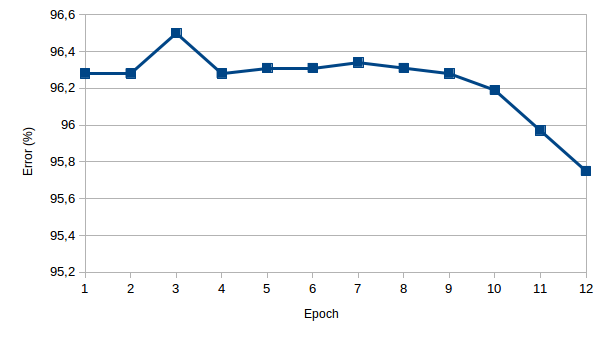
\includegraphics[width=0.7\textwidth]{images/epoch_LFW.png}
\caption{Error of Lenet using LFW.} \label{fig:LENETLFW}
\end{figure}

Figure \ref{fig:LENETLFW} represents the validation error \% in each epoch, and it could be seen that in the last epoch, the error is the smallest one, and the test error in that point is 95.125000 \%, a really high error rate because of the bag learning procedure.\\

\subsubsection{Changing learning rate}
Despite the fact that the configuration of the networks is not to this database, learning rate is going to be changed so it is possible to know how it affects.\\

In order to know how the net works with different learning rates, it has been changed to 0.001 and the number of epoch has been raised to 50.\\

The error at validating in each epoch could be seen in figure \ref{fig:LENETLFWerror0-001} , where it is shown that the net does not learn because the learning rate is too small and it would need more epochs. The cost function at training of the training could be seen in figure \ref{fig:LENETLFWcost0-001}, where the cost it has been reducing during epochs, but it has not been reduced significantly, from 8.7 to 8.1.\\

\begin{figure}[htb]
\centering
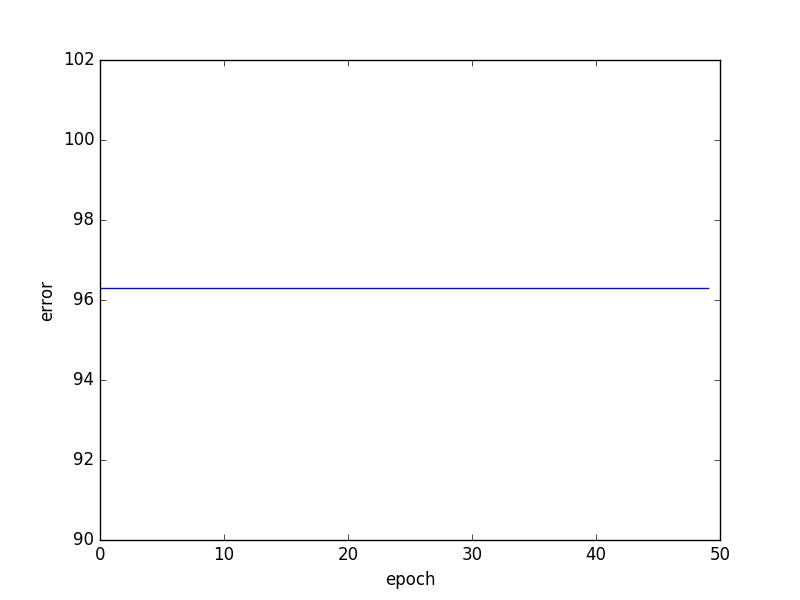
\includegraphics[width=0.7\textwidth]{images/LFW_learningrate/error_0_001.png}
\caption{Error of LeNet-5 using LFW with a learning rate of 0.001.} \label{fig:LENETLFWerror0-001}
\end{figure}

\begin{figure}[htb]
\centering
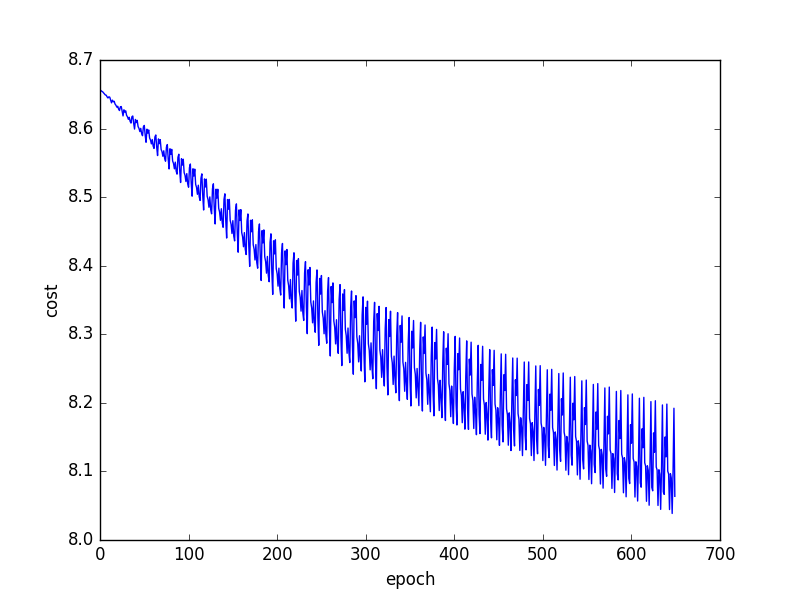
\includegraphics[width=0.7\textwidth]{images/LFW_learningrate/cost_0_001.png}
\caption{Cost of Lenet using LFW with a learning rate of 0.001.} \label{fig:LENETLFWcost0-001}
\end{figure}

A 97,73\% error of test performance has been gotten, which has been obtained in iteration 13. \\

The conclusion is the learning rate is too small to this configuration of the net and the data given.\\

If the learning rate is increased to 0.01: Best validation score of 96.266667 \% obtained at iteration 481, with test performance 95.733333 \%\\

\begin{figure}[htb]
\centering
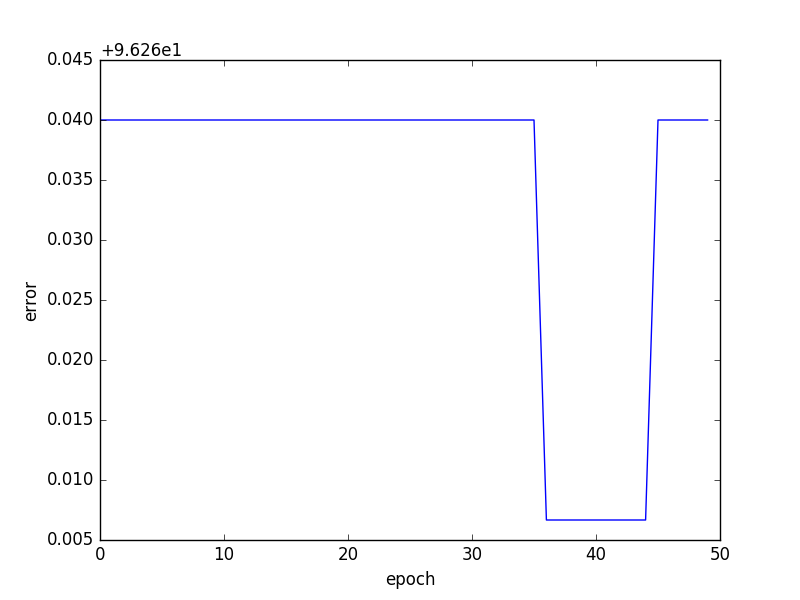
\includegraphics[width=0.7\textwidth]{images/LFW_learningrate/error_0_01.png}
\caption{Error of Lenet using LFW changing learning rate to 0.01.} \label{fig:LENETLFW_lr0_01}
\end{figure}

If learning rate is increased to 0.1:Best validation score of 96.300000 \% obtained at iteration 13, with test performance 95.733333 \%\\

\begin{figure}[htb]
\centering
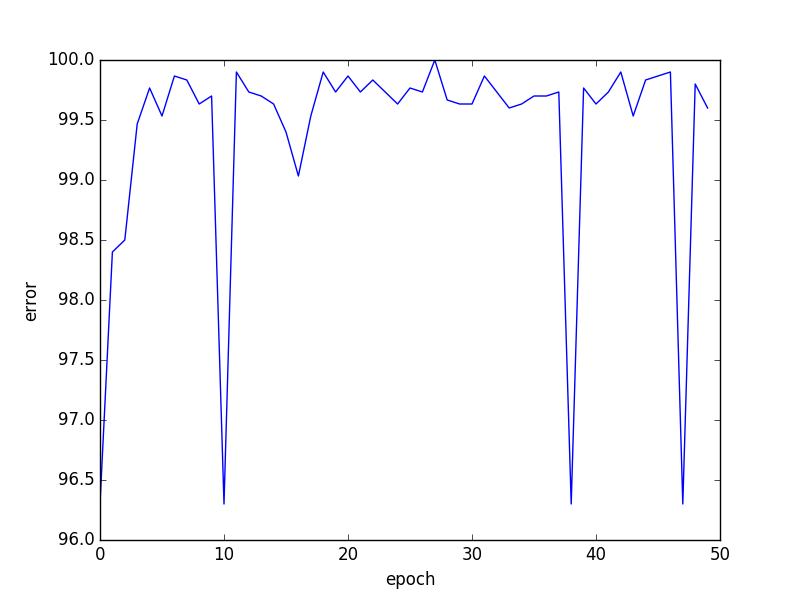
\includegraphics[width=0.7\textwidth]{images/LFW_learningrate/error_0_1.png}
\caption{Error of Lenet using LFW changing learning rate to 0.1.} \label{fig:LENETLFW_lr0_1}
\end{figure}

If learning rate = 0.5 Best validation score of 96.3 \% obtained at iteration 143, with test performance 95.73\% \\

\begin{figure}[htb]
\centering
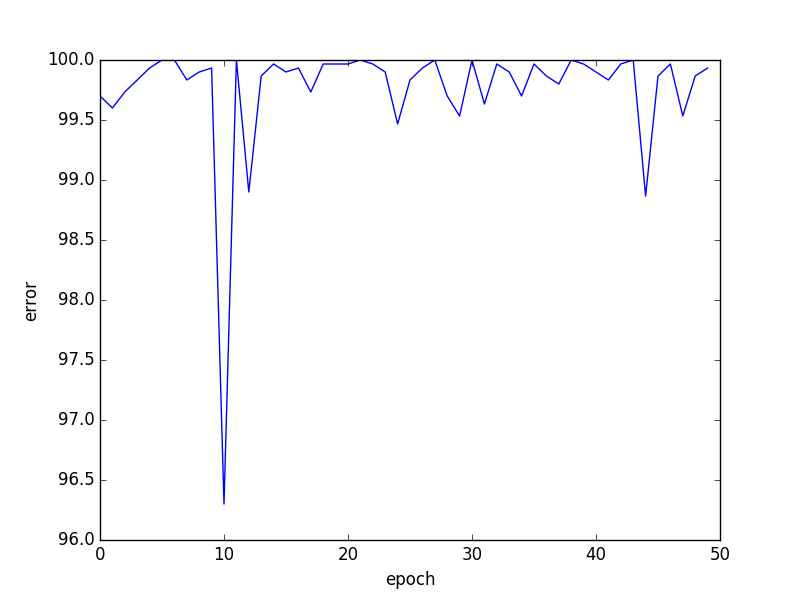
\includegraphics[width=0.7\textwidth]{images/LFW_learningrate/error_0_5.png}
\caption{Error of Lenet using LFW changing learning rate to 0.5.} \label{fig:LENETLFW_lr0_5}
\end{figure}

In conclusion, if the learning rate is too big, the network do not get a optimal minimum and if the learning rate is too small it takes too mch iteration to learn or getting to to optimal minimum.\\


\subsubsection{Changing convolutional parameters}
Convolutional layers are built with the Theano function \textit{theano.tensor.nnet.conv2d}. The size of convolutional layers depends on the number of filters that users would like, the dimension of images, it is not possible to use the same convolutional layer for 3d images (rgb) than grey scale images (1 dimension), and also depends on the high and width user would like to give.\\

The output of a convolutional layer depends on the size of the filter and the size of input images. At the output, a new bunch of images are created from the input images and the characteristics of the layer.\\

Also, it is important to consider the batch size, because the layer is not fed by a individual image; the layer is fed by the bunch of images.\\

Lets have a bit of fun with convolutional layers, the number of filters and the size of them it is going to be changed. A learning rate of 0.1 is going to be used for 50 epoch.\\

In the first example, the number of filters of the first layer is going to be increased from 20 to 40, and the number of the second layer from 40 to 60.

In figure \ref{fig:LENETLFW_ker1} could be seen the error which has been gotten in each epoch, where the best vest validation score of 94.9\% has been obtained at iteration 559, with test performance 95\%.

\begin{figure}[htb]
\centering
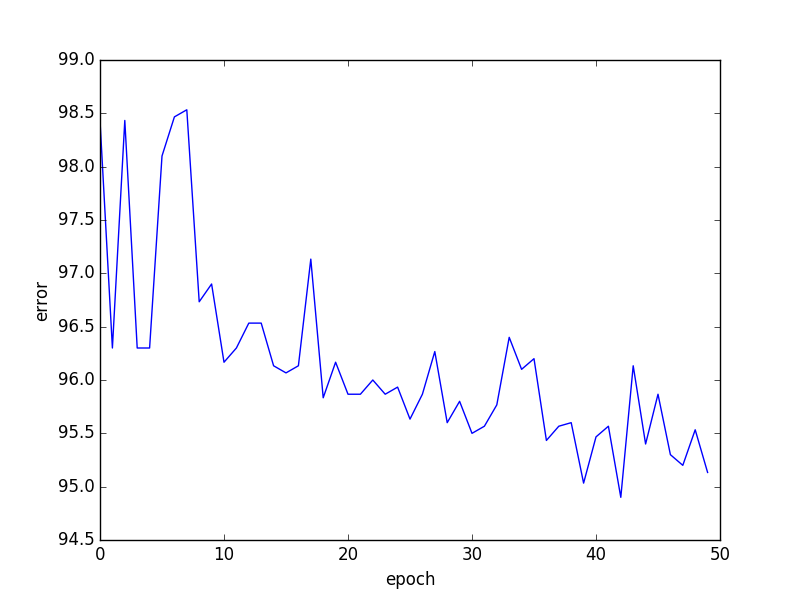
\includegraphics[width=0.7\textwidth]{images/LFW_layers/error_conv_40_60.png}
\caption{Error of Lenet using LFW changing number of kernels in example 1.} \label{fig:LENETLFW_ker1}
\end{figure}

If the number of filters has been increased, the time that the code takes to run is increased significantly. Also, the results of the network changes, this is a parameter that should have in consideration.\\

Also, it is possible to modify the filter shape, in the previous examples, the size of both kernels were 5x5, in this example, the second one, the first convolutional layer would have a filter size of 3x3, the second one would keep its original size.\\

\begin{figure}[htb]
\centering
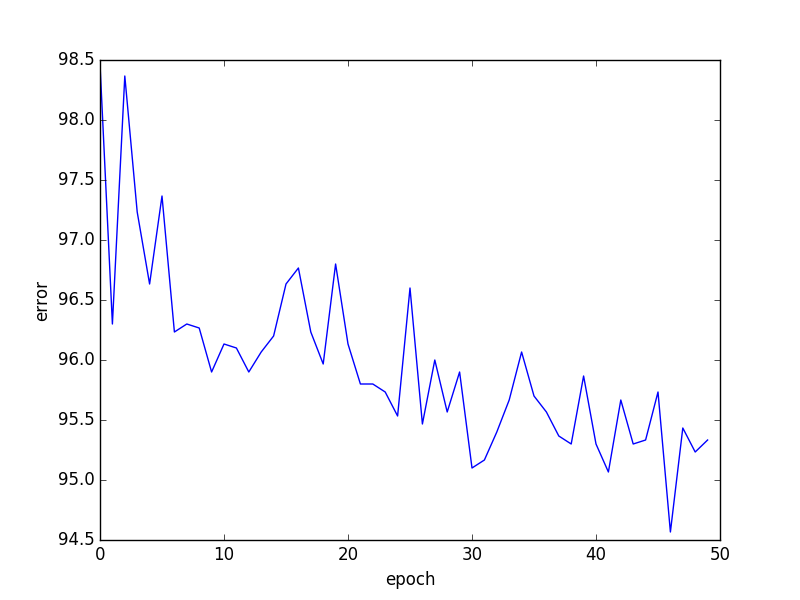
\includegraphics[width=0.7\textwidth]{images/LFW_layers/error_conv_40_60_2.png}
\caption{Error of Lenet using LFW changing number of kernels and the filter size in example 2.} \label{fig:LENETLFW_ker2}
\end{figure}

It is interesting seeing how the error of the network has been improved when the number of kernels has been changed and, in this example, has been improved too when the size of the filter has been changed.\\

The error in each epoch of this example could be seen in figure \ref{fig:LENETLFW_ker2}, where the best validation score obtained has been 94.567\% error iteration 611, with test performance error 93.967\%.\\

In order to see the difference between using a big size filter and one of a small size, in the next example, third example, 40 and 60 kernels are going to be used, and the size of each one is 3 and 10 for layer 0 and layer 1 respectively. In epoch number 40, the weighs of each layer has been saved and in figure X are represented. At irst sight, it is possible to see that with a big size.\\

\begin{figure}[htb]
\centering
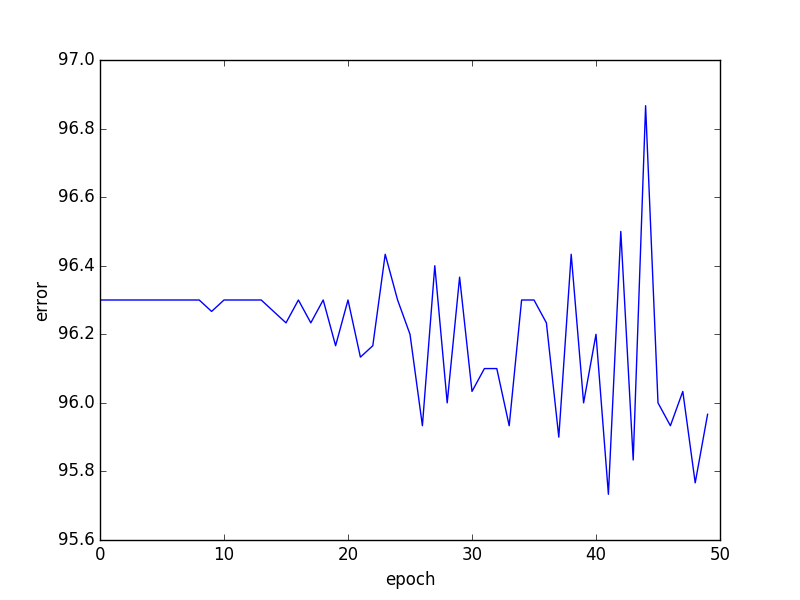
\includegraphics[width=0.7\textwidth]{images/LFW_layers/error_conv_40_60_3.png}
\caption{Error of Lenet using LFW changing number of kernels and the filter size in example 3.} \label{fig:LENETLFW_ker3}
\end{figure}

Also, it is possible to see the output at the convolutional layer, in figure \ref{fig:LENETLFW_ker4}, the first 25 output images are shown for both layers.\\

\begin{figure}[htb]
\centering
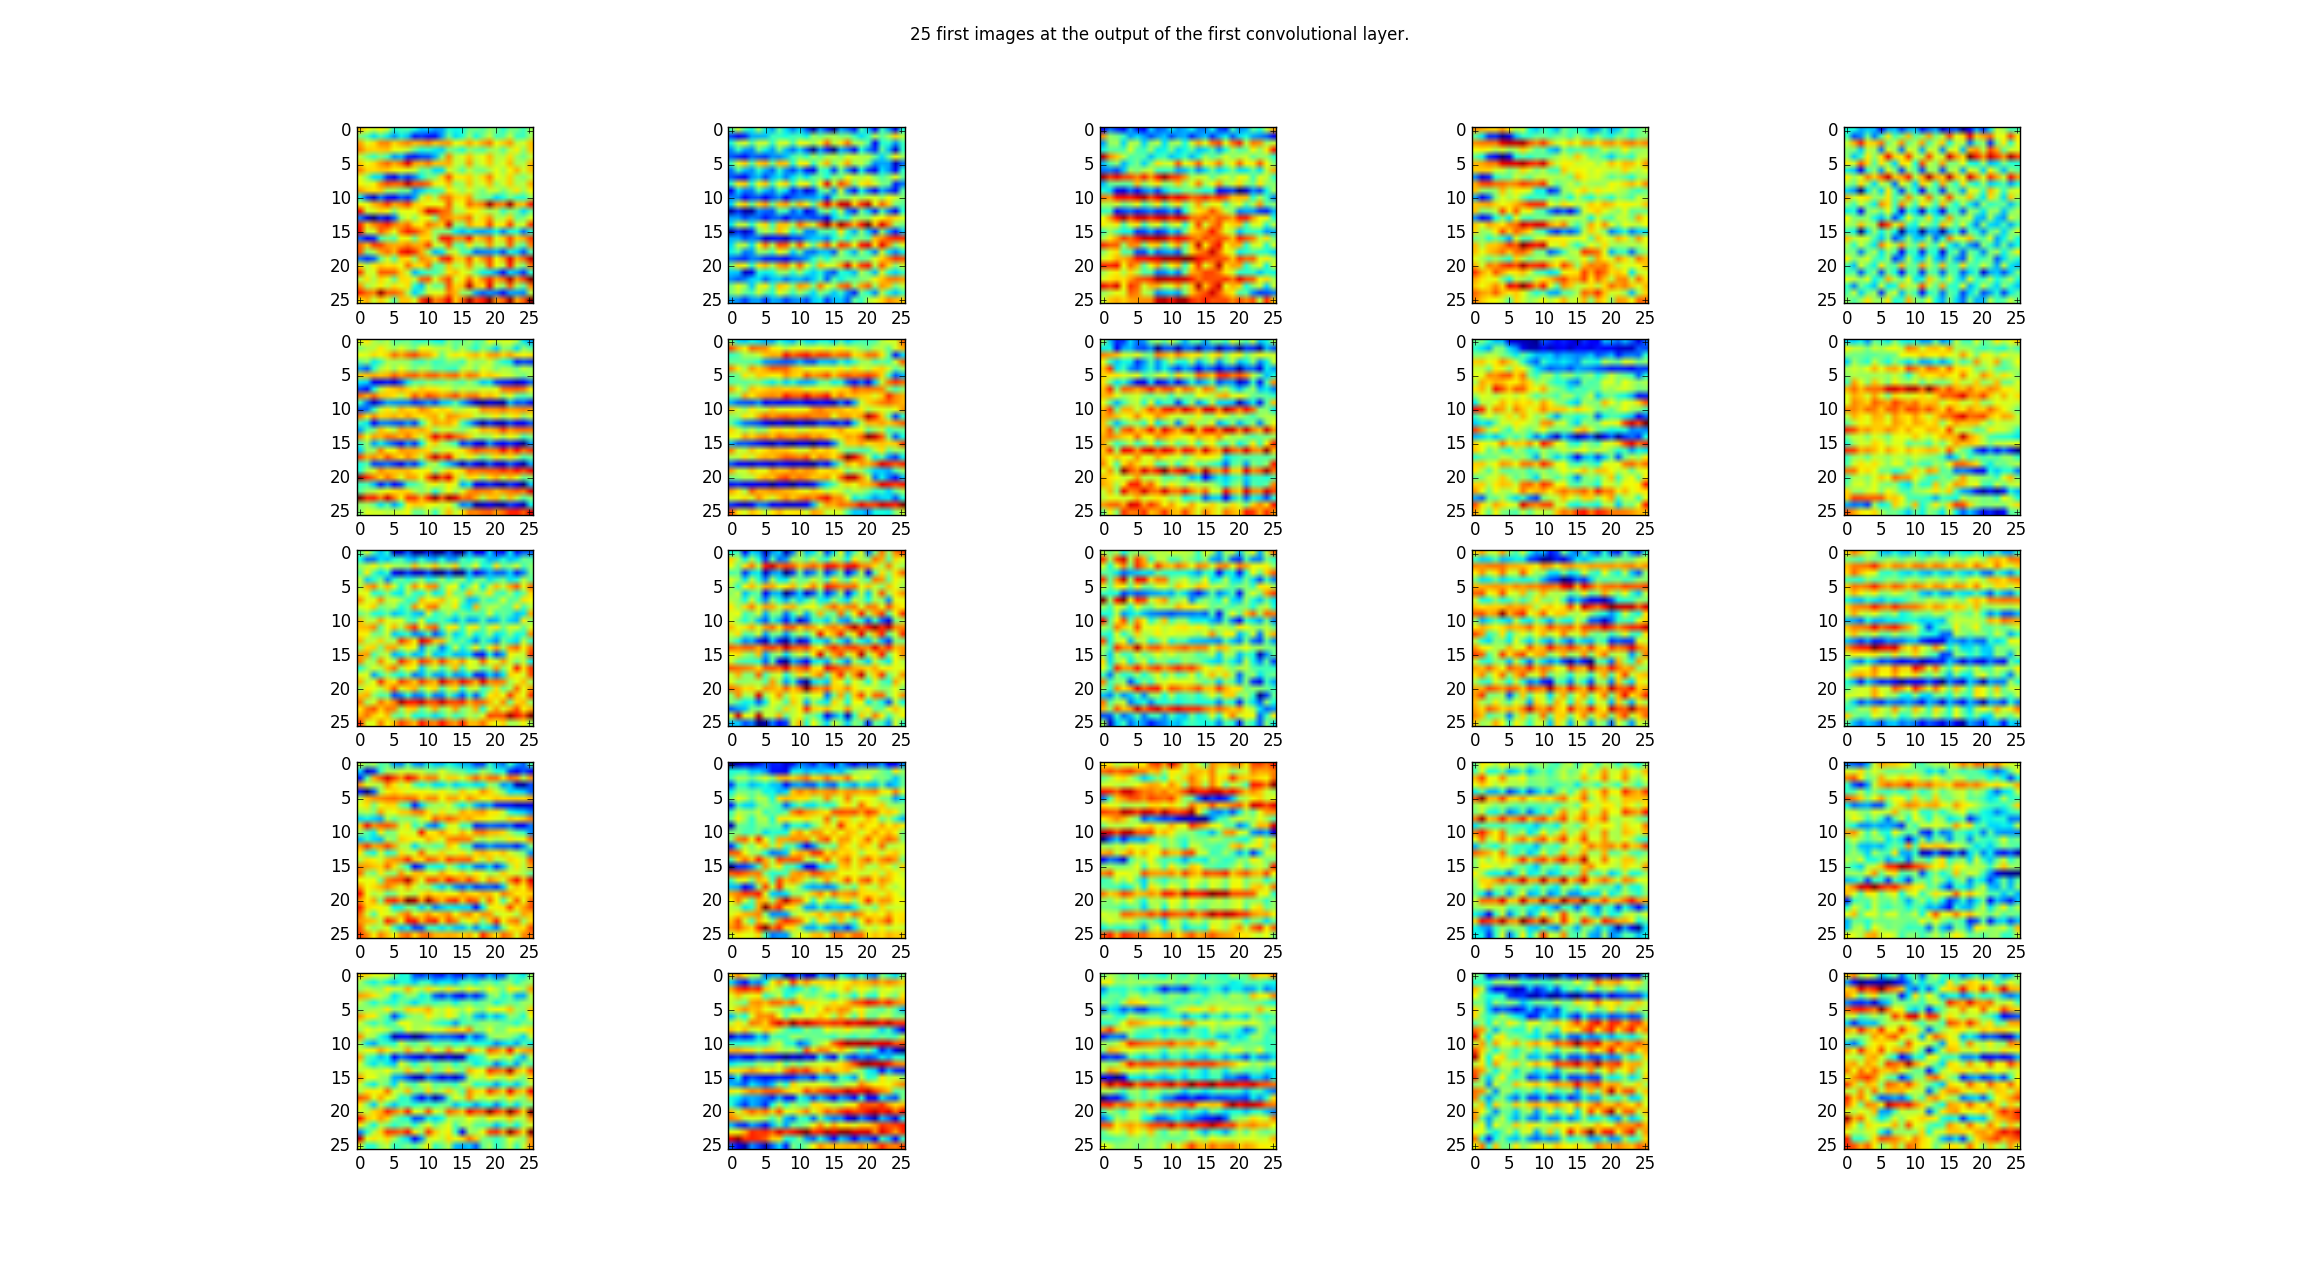
\includegraphics[width=1.4\textwidth]{images/LFW_layers/conv_0_out.png}
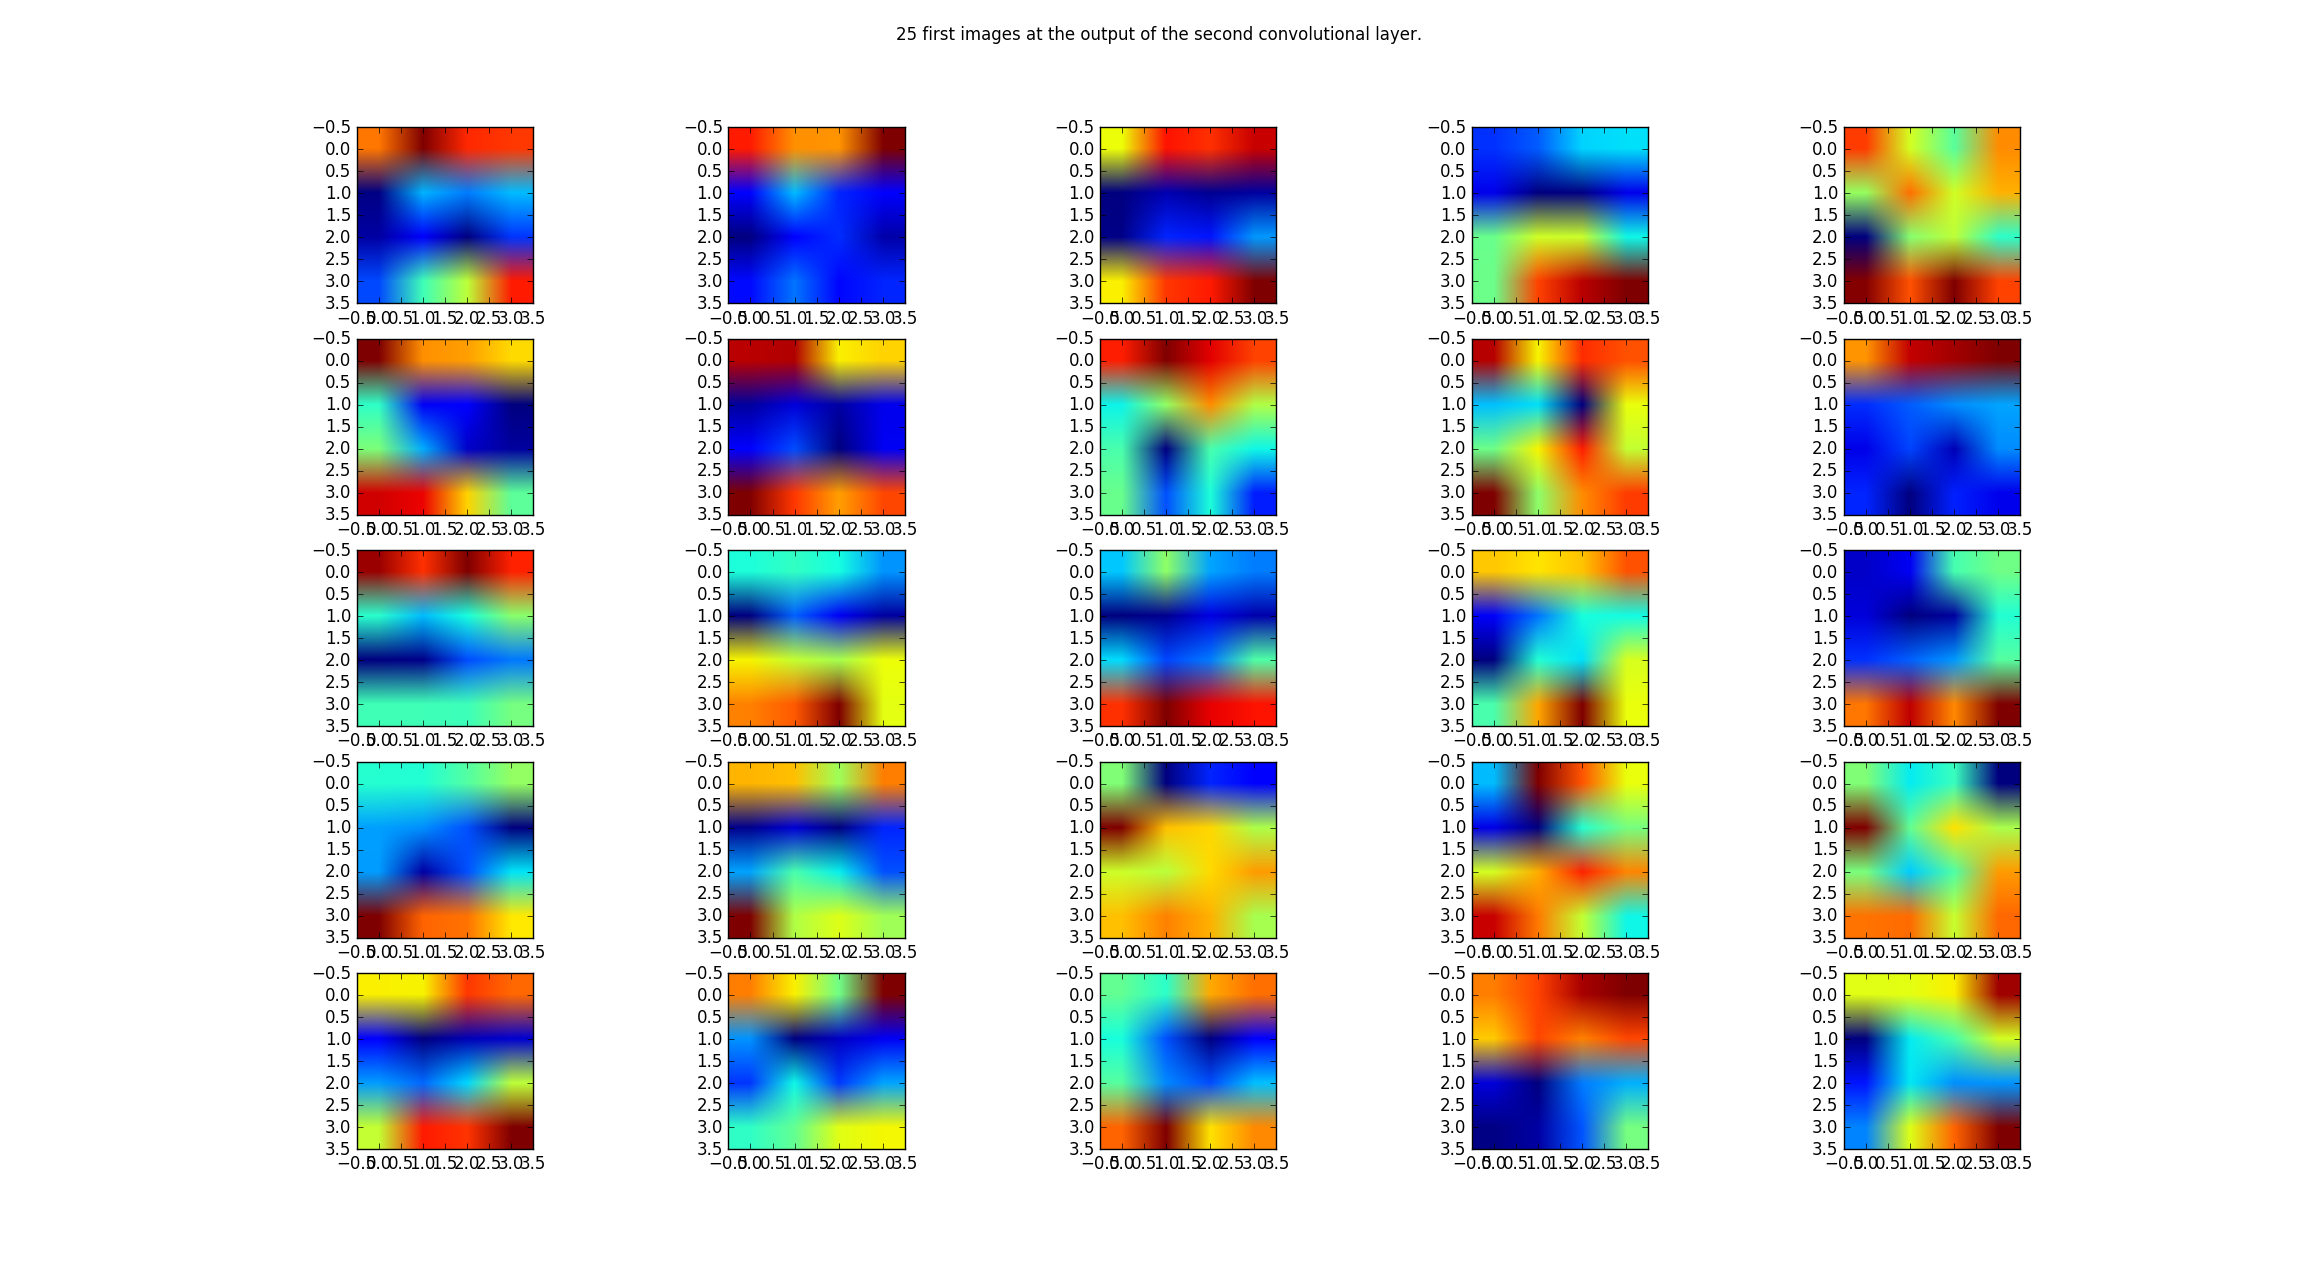
\includegraphics[width=1.4\textwidth]{images/LFW_layers/conv_1_out.png}
\caption{Output of the convolutional layers using LeNet and LFW.} \label{fig:LENETLFW_ker4}
\end{figure}

The result of the third example is a best validation score of 95.73 \% obtained at iteration 546, with test performance 95.23 \%. \\

The cost function of those three experiments are represented in \ref{fig:LENETLFW_Cost}

\begin{figure}[htb]
    \centering
        \subfigure[Example 1]{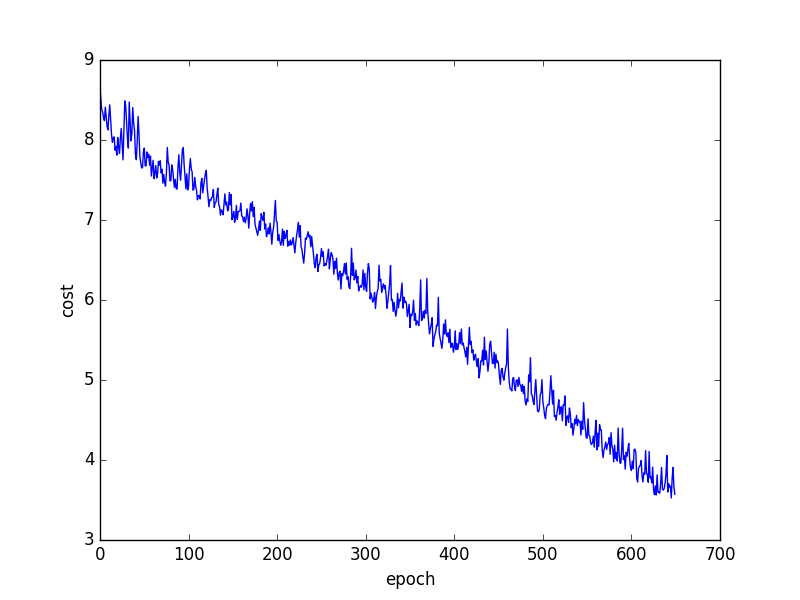
\includegraphics[width=0.47\textwidth]{images/LFW_layers/cost_conv_40_60.png}}
        \subfigure[Example 2]{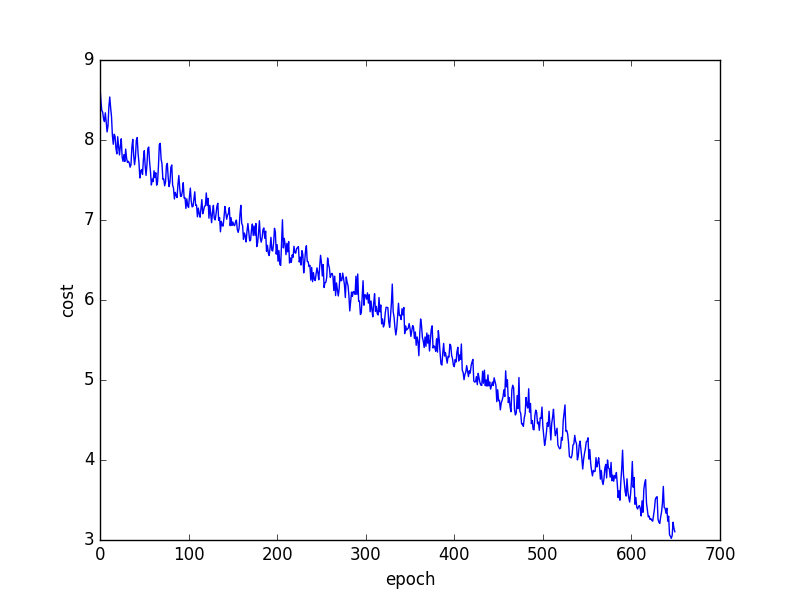
\includegraphics[width=0.47\textwidth]{images/LFW_layers/cost_conv_40_60_2.png}}
		\subfigure[Example 3]{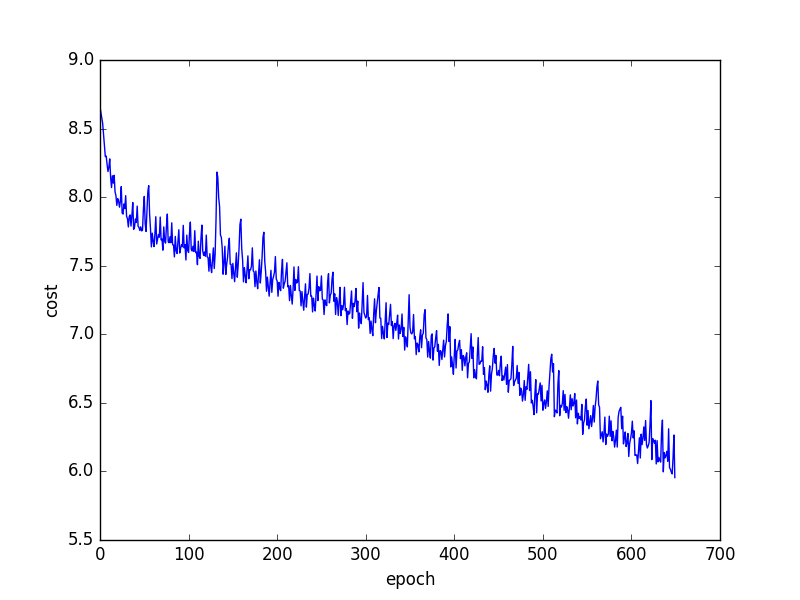
\includegraphics[width=0.47\textwidth]{images/LFW_layers/cost_conv_40_60_3.png}}

    \caption{Cost function at training of the three examples chanching the convolutional parameters.} \label{fig:LENETLFW_Cost}
\end{figure}

%\subsubsection{Changing pooling parameters}
%The theano function used to build this kind of layer depends of theano version,


\subsubsection{Using ReLu as an activation function instead of tanh}
Originally LeNet uses as activation function tanh(), but in this section, ReLu (Rectified linear units) activation function is going to be used. In equation \ref{Relu-formula} is shown how it is defined.  \\

\begin{equation}
f(x) = max(0,x)
\label{Relu-formula}
\end{equation}

The error and the cost in each epoch could be seen in figure \ref{fig:LENET_relu}

\begin{figure}[htb]
\centering
		\subfigure[Cost at training]{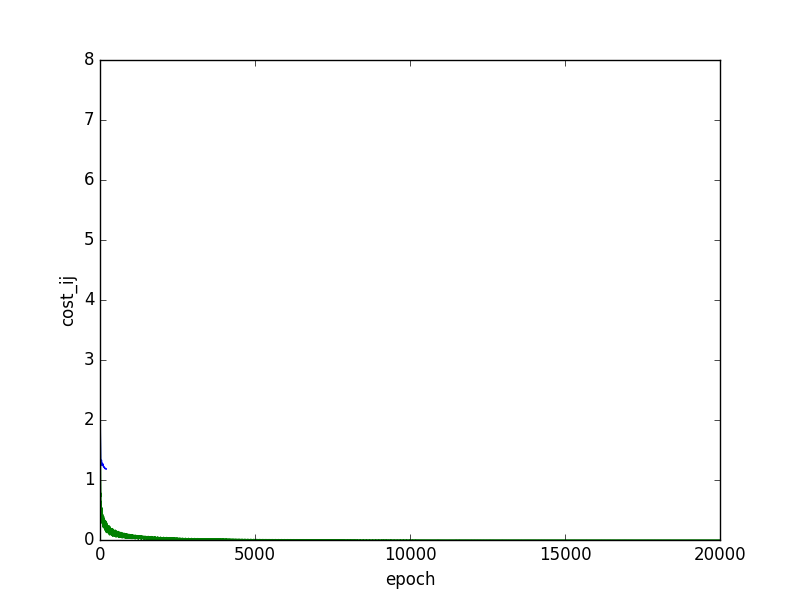
\includegraphics[width=0.47\textwidth]{images/images_lenet/cost_relu.png}}
		\subfigure[Error at validation]{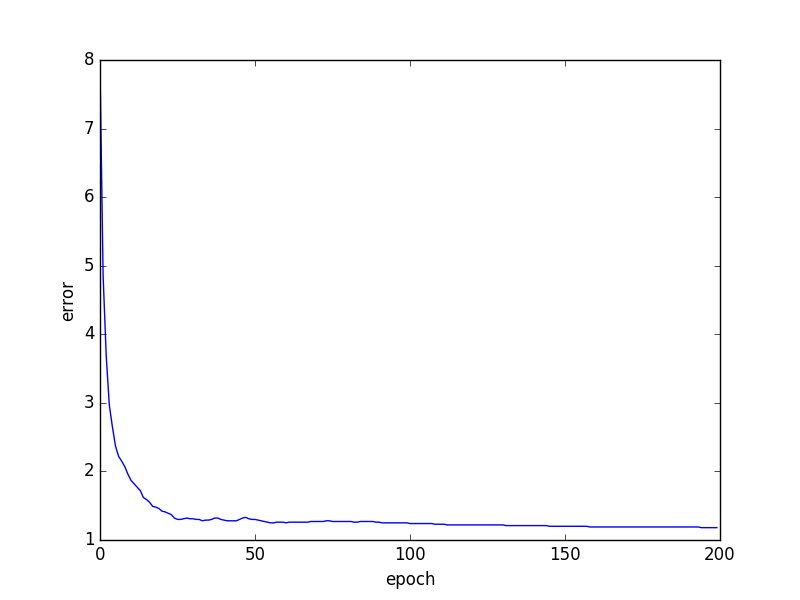
\includegraphics[width=\textwidth]{images/images_lenet/error_relu.png}}

\caption{Error and cost using ReLu instead of tanh}
\label{fig:LENET_relu}
\end{figure}

\subsection{Using FRAV dataset}
One of the databases used with the final architecture and configuration of the network is FRAV database. LeNet-5 is tested with this database in this current section.\\

The experiments made with this database are just with RGB images, so 939 images of people has been used, 489 samples are used for the training subset, 162 samples has been used in the validation subset and 279 samples in the test subset.\\

Because images has not the same shape, they have been re-sized into 252x180, this new shape is proportional 0.7*height = weight because all images studied save that proportion. In addition, making images smaller also gives the security of not having memory problems, because the huge quantity of used images.\\

The network has been tested with this databases in the two ways of classify images, with two classes (genuine and attacks) and five classes (genuine and four classes, one per type of attack).\\ %Also, different learning rates have been used.\\

The first experiment made was based in the neural network LeNet, without changing parameters, but batch size because 500 is too big, there are not enough samples:\\

\begin{itemize}
\item 25 epoch.
\item 20 and 50 kernels of each convolutional layer.
\item 50 batch size.
\item 0.01 learning rate.
\item Logistic regression with 10 neurons.\\
\end{itemize}

The obtained results are with 5 classes classification and there were not as bad as the one with labeled faces in the wild (LFW), in this database there are more samples per class.\\

Figure \ref{fig:FRAV_five} shows the validation error of five classes, the best validation error has token place in epoch 7 with test performance 60.4\%. It has token 68.78 minutes to run.\\

\begin{figure}[htb]
\centering
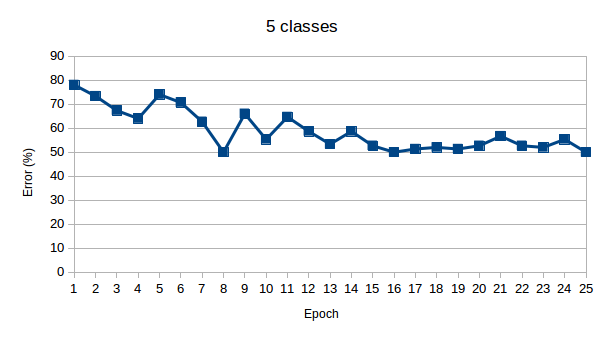
\includegraphics[width=0.7\textwidth]{images/epoch_5classes_FRAV_1.png}
\caption{Error using FRAV database and five classes.}
\label{fig:FRAV_five}
\end{figure}

In figure \ref{fig:FRAV_two}, the validation error in different epoch could be visualized using two classes to classify. It could be seen that in each epoch the validation error is the same. Test error performance at the first epoch is 23.2 \%. The total time of the running has been 64.0167 minutes.\\

\begin{figure}[htb]
\centering
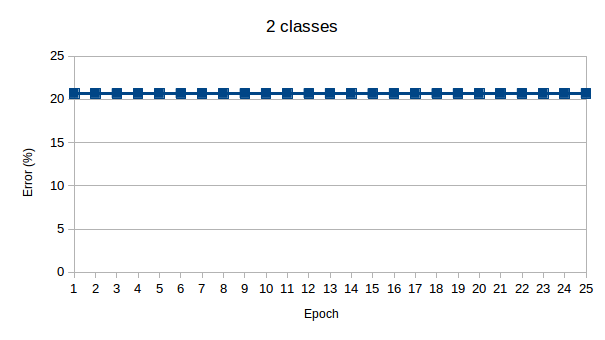
\includegraphics[width=0.7\textwidth]{images/epoch_2classes_FRAV_1.png}
\caption{Error using FRAV database and two classes.}
\label{fig:FRAV_two}
\end{figure}

The time in both cases, classifying with two or five classes are similar, but not the result, is better when just two classes are used and no differentiation is made among attacks. There would be need more samples and more time to get a better score if five classes classification is wanted.\\

% TODO For the time being no differentiation among classes is done, there is no necessity to differentiate the attacks, so the classification is going to be bi-classe: genuine and attack.\\

\section{Defining a new architecture}
From the LeNet-5 code, which is proportioned by \url{deeplearning.net}, changes has been developed to build a new architecture \cite{LSTM-CNN}. \\

%After this, the CNN has been changed in order to build a CNN similar to the one described in \textit{Learning Temporal Features Using LSTM-CNN Architecture for FaceAnti-spoofing}.\\

The new architecture of the Convolutional Neural Network is formed by two convolutional layers, the first one with 48 filters and the second one with 96. The size of the filters is 5x5. Each convolutional layer is followed by a max pool layer of size 2x2.\\

The activation function has been changed to the rectified linear activation function (ReLu), a function implemented in Theano has been used to this purpose \textit{theano.tensor.nnet.relu}. For the weight initialization, a normalized distribution of weights and bias, the same which was implemented in LeNet-5: weights are sampled randomly from a uniform distribution.\\

Because of the huge number of images, the  batch size has been changed to 20. And the learning rate is 0.001. The number of neurons at the output of the hidden layer are 100. The classifier is the sigmoid function. 25 epoch have been used for training the network.\\

the used database in this experiment is Casia database and its samples have been pre-processed, images are resized into 52x104, the relation between width and height is proportional to the original size of images, but they have not the same shape. At the time to split the data into train, test and validation, different seeds have been used with the purpose of test the net with different combination of the data.\\

% NO ENCUENTRO LOS RESULTADOSS
%(AÑADIR LOS RESULTADOS CON LAS DIFERENTES SEMILLAS)

%\subsection{using CASIA dataset}
%Before proving casia databse in the convolutional neural network, the net has been modified in order to diference training and test, so the net train and validate and when a new best score of error is gotten, the network is saved. After training, the best configuration of the network is loaded and tested with the test set.\\

two different ways of using classes has been used, first, two classes has been used, one the imges of the genuine people and another class with the atacks, the last way of separate classes is assigning one different class to a different attack.\\

%Casia database has also been proved using two classes and two seeds.\\

%(AÑADIR LOS RESULTADOS)


\section{Regenerating the databases}
The databases have been generated in a different way from the used before. In this new way, the possibility of access to the misclassified samples is possible. SO the characteristic of misclassified images could be studied. This is not used now, but in the future it could be useful.\\

In order to build the new database, a script as been programmed manually because the test-train split sklearn function does not let know what image has been read and now it is possible to compare the right class of each image with the predicted one.\\

All this work has been changed because it is interesting to know the characteristics of people (if has beard, glasses or long hair) that are not well classified.\\

It has been necessary to shuffle the data twice in order to mix it properly and training, testing and validating test would have data of the five classes.\\

\subsubsection{Adding images in characteristic level}
In order to get this particular goal, each image is re-sized proportionally to original image to 52x104 dimensions. Each NIR image is appended to its correspondent RGB image.\\

In order to create a list of images where images are not putted in order, each image followed by another could be of a different class. Two shuffles has been necessary, the first one with a seed = 0.5 and the second one with a seed = 0.1, so the randomize order of images could be repeated.\\

For training, the 70\% of the total data has been used, for testing the 20\% and for validating the testing 10\%. There are 157 images in each class and the distribution is represented in the table \ref{FRAV_distribution1}.\\

\begin{table}[htb]
\centering
\label{FRAV_distribution1}
\begin{tabular}{c|ccccc|c|}
\cline{2-7}
                                     & \multicolumn{1}{c|}{Class 0} & \multicolumn{1}{c|}{Class 1} & \multicolumn{1}{c|}{Class 2} & \multicolumn{1}{c|}{Class 3} & Class 4 & Total of samples \\ \hline
\multicolumn{1}{|c|}{Training set}  & 94                           & 119                          & 116                          & 145                          & 76      & 550              \\ \cline{1-1}
\multicolumn{1}{|c|}{Testing set}    & 33                           & 38                           & 37                           & 7                            & 42      & 157              \\ \cline{1-1}
\multicolumn{1}{|c|}{Validating set} & 30                           & 0                            & 4                            & 5                            & 39      & 78               \\ \hline
\end{tabular} \caption{Distribution of samples FRAV (RGB + NIR) database}

\end{table}

The code runs for 150 epoch with a learning rate of 0.001 and a batch size of 20 images.\\

The disadvantage of using mini-batches is that there are some images remain and the quantity of less than a mini-batch, that images are not used, so from 157 testing images, just 140 has been used.\\

The test error that has been gotten is 30\% at iteration 1863 where the best validation score was gotten (26,67\%). Where:

\begin{itemize}
\item Class 0 has been misclassified  14 times
\item Class 1 has been misclassified  6 times
\item Class 2 has been misclassified  7 times
\item Class 3 has been misclassified  2 times
\item Class 4 has been misclassified  2 times
\end{itemize}

To get that results 3,04 hours was needed to run the code.\\

%y_pred = [2,4,2,1,2,1,2,1,4,0,3,1,2,1,2,0,2,0,3,1,3,1,3,1,2,1,2,1,4,1,2,4,2,1,2,1,2,1,2,1,2,1,3,1,2,1,2,0,2,1,2,1,3,1,2,1,2,1,3,1,4,1,2,1,2,1,2,1,3,1,2,1,2,1,2,1,0,4,3,4,0,1,1,4,1,4,1,4,2,4,0,4,1,4,0,4,1,4,2,4,1,4,1,1,0,4,0,4,2,4,0,4,1,4,0,4,0,4,3,4,4,4,0,4,1,4,4,4,2,4,0,4,1,4,1,4,1,4,3,4]

%y_real = [2,1,2,1,2,1,2,1,4,1,2,1,2,1,2,1,2,1,3,1,2,1,2,1,2,1,2,1,4,1,2,1,2,1,2,1,2,1,3,1,2,1,2,1,2,1,2,1,2,1,2,1,2,1,2,1,2,1,3,1,2,1,2,1,2,1,2,1,2,1,2,1,2,1,2,1,0,4,3,4,0,4,0,4,0,4,0,4,2,4,0,4,0,4,0,4,0,4,3,4,0,4,0,4,0,4,0,4,2,4,0,4,0,4,0,4,0,4,3,4,0,4,0,4,0,4,0,4,2,4,0,4,0,4,0,4,0,4,3,4,0,4,0,4,0,4,0,4,2,4,0,4,0,4,0,4,0]


%\section{Metrics}
%In order to measure the net and its works, some metrics would be used, but %to do that, the data has to be splited in other way because with the %function train\_test\_split there is no chance, which is know, to get the %image if it is not printed; so a own method has been developed and it is %posible too pseudo-randomize the data.\\

%The metrics that has been used are:
%\begin{itemize}
%\item FAR: False aceptance rate
%\item FRR: False rejection rate
%\end{itemize}

\clearpage

\subsection{Architecture implemented in CASIA videos}
In this section, the architecture used in the paper of the CASIA videos would be repeated partially. The paper is learn convolutional neural network for face anti-spoofing.\\

The architecture followed in the paper is the same used in Imagenet, it is formed by five convolutional layers, followed by three fully-connected layers. The two first conv layer and the last one are followed by a max-pool layer. The two first conv layers are followed by response normalization layers too. Authors use ReLu like activation function in each layer. The first two fully-connected layers are followed by two dropout layers, and the last layer output is followed by softmax layer as a classifier.\\

Authors do not explain anything else about the architecture. In the paper of Imagenet is said that:

\begin{itemize}
\item The ReLU non-linearity is applied to the output of every convolutional and fully-connected layer.
\item The first convolutional layer filters the 224×224×3 input image with 96 kernels of size 11×11×3 with a stride of 4 pixels.
\item The second convolutional layer takes as input the (response-normalized and pooled) output of the first convolutional layer and filters it with 256 kernels of size 5 × 5 × 48.
\item The third, fourth, and fifth convolutional layers are connected to one another without any intervening pooling or normalization layers.
\item The third convolutional layer has 384 kernels of size 3 × 3 × 256 connected to the (normalized, pooled) outputs of the second convolutional layer.
\item The fourth convolutional layer has 384 kernels of size 3 × 3 × 192.
\item  The fifth convolutional layer has 256 kernels of size 3 × 3 × 192.
\item The fully-connected layers have 4096 neurons each.
\item The maxpool size filter si 2x3 because it reduces the error 0.4\% - 0.6\% compared to 2x2 filters.
\item In Imagenet uses 224x224 images.
\end{itemize}

It is not explained how authors change the architecture of Imagenet.\\

The data used to this experiment is the Casia database, the one that uses in the paper, although authors, use Reply-attack too.\\

The data is composed by two folders, a training folder and a test data, in each folder there are some user folders, in each user folders there are two videos from the real user, tho videos of the user with a mask, two videos with the mask and with a hole in the eyes and two videos with a digital screen where a user is shown in the screen. 3 attacks are presented, so four classes are used (real users, users with mask, users with mask and eyes and a digital screen). It is not specified how many frames authors use, so it s supposed that they use all the video.\\

For each frame, the face is looked for in the image with viola jones algorithm implemented in opencv, and the image is cropped and saved, but in that image cropped there is no background, so different scales, 1.4, 1.8, 2.2, 2.6, are used to get background, because in learn convolutional neural network for face anti-spoofing and then images are re-sized to 128x128.\\

In order to carry out this experiment, a better computer has been needed because it was no possible to run with the same that the utilized in the previous experiments.\\

But with a better computer, it is not possible read more than 2 or 3 frames per video to run the net, because it has a huge architecture with a big quantity of filters per layer.\\

So the experiment with the videos has not been possible to be carried out.\\

In addition, is it not possible to carry out the architecture of imagenet with the size of Casia images because if it is started with 128x128 images, at the end,  images sizes are images of < 1px.\\

In order to know how strides work, a python file has been created called understanding strides, in which a pickle format file is loaded. This pickle format file is the output of a layer, and it is possible to see the size of images of the layer. So it is possible to know the size of images after striding and this number could be saved to be written in the conv layer.\\

In this computer, the theano function used to build the max\-pool layer has changed bacuse of Theano version, the previous function used in Theano  \textit{theano.te\-nsor.sig\-nal.down\-sam\-ple.max\-\_pool\_2d} has been replaced by \textit{thea\-no.ten\-sor.sig\-nal.pool.pool\_2d} using the mode \textit{max}.\\

To  sum up, In this first experiment, the architecture is formed by the convolutional and pooled out layers but without strides. The folder where this experiment has been developed has been in frav\_casia\_imagenet. The architecture is just based in conv, pool and hidden layer (no dropout, softmax or normalization layer). In figure \ref{fig:error_imagenet1} it is possible to see how the error is descending in each epoch and get stabilized with a 5\% aprox. error. \\
\begin{figure}[htb]
\centering
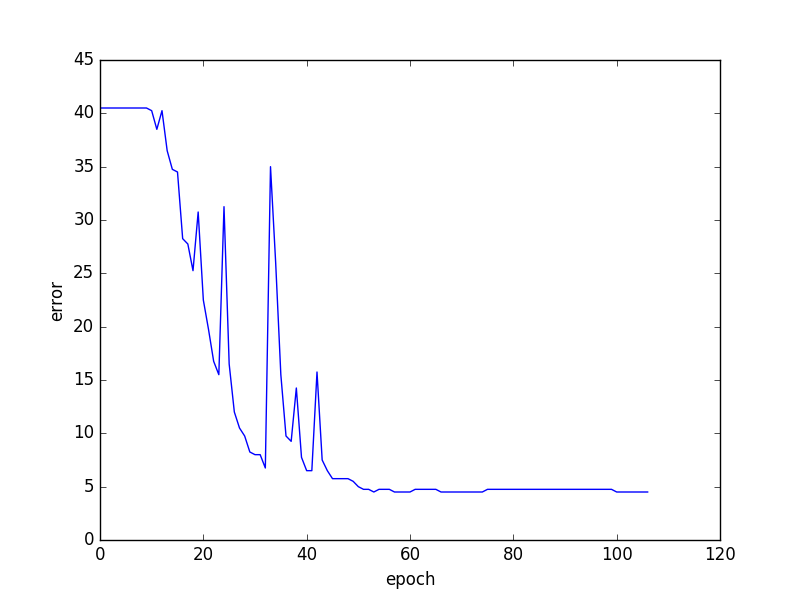
\includegraphics[width=0.7\textwidth]{images/imagenet/error_frav-Imagenet1.png}
\caption{Error of Lenet in the first try to build imagenet.} \label{fig:error_imagenet1}
\end{figure}

The code had been running for 364,39 hours. And the true positive rate, true negative rate, false positive rate and false negative rate are available in table \ref{tabla_error_imagenet1}. \\

\begin{table}[htb]
\centering
\label{tabla_error_imagenet1}
\begin{tabular}{lllll}
\cline{1-4}
\multicolumn{1}{|l}{TP} & \multicolumn{1}{l}{TN} & \multicolumn{1}{l}{FP} & \multicolumn{1}{l|}{FN} &  \\ \cline{1-4}
\multicolumn{1}{|l}{156} & \multicolumn{1}{l}{623} & \multicolumn{1}{l}{10} & \multicolumn{1}{l|}{11} &  \\ \cline{1-4}
                         &                         &                         &                         &  \\
                         &                         &                         &                         &
\end{tabular}
\caption{TP, TN, FP, FN rates in the first trying of imagenet.}

\end{table}

\clearpage
%\subsection{Reading frav faces}
%He hecho un base de datos generator, en el que voy creando la base de datos, dentro de esa carpeta hay un info en el que se explica como se leen las imagenes. Puedes escalarlas, puedes buscar caras o no y en guardarlas en distintas escalas como en casia.\\
